% TODO: sửa lại theo mục đích của luận văn, focus vào những lỗ hổng nào mà viết
\section{Các thành phần quan trọng về bảo mật của ứng dụng web}
\subsection[Thông điệp HTTP]{Thông điệp HTTP}
Giao thức truyền tải siêu văn bản (hypertext transfer protocol - \acrshort{http}) là giao thức ứng dụng bất đồng bộ, không trạng thái (stateless) phổ biến nhất dùng để truyền tải dữ liệu qua lại giữa người dùng (client) và máy chủ (server). Có hai loại thông điệp \acrshort{http} là thông báo yêu cầu và thông báo phản hồi HTTP, được mô tả như Hình \ref{fig:http} dưới đây:
\begin{figure}[H]
  \centering
    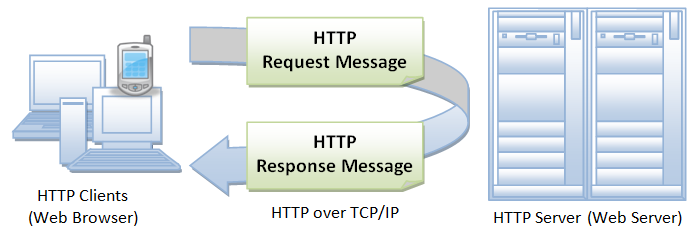
\includegraphics[width=\textwidth,keepaspectratio=true]{images/http.png}
  \caption[Hai loại thông điệp HTTP]{Hai loại thông điệp \acrshort{http}\protect\footnotemark}
  \label{fig:http}
\end{figure}
\footnotetext{Nguồn: https://www.ntu.edu.sg/home/ehchua/programming/webprogramming/HTTP\_Basics.html}
\textbf{Thông báo yêu cầu HTTP} (HTTP request) được gửi từ người dùng đến máy chủ để yêu cầu máy chủ thực thi một hành động nào đó. \acrshort{http} request gồm các thành phần:
\begin{itemize}
    \item \textbf{Dòng bắt đầu (start line)} ví dụ như \colorbox{gray!30}{\texttt{POST / HTTP/1.1}}, \colorbox{gray!30}{\texttt{GET /1-duck.png HTTP/1.0}},\\\colorbox{gray!30}{\texttt{HEAD /items.html?productId=1337 HTTP/1.1}}, \colorbox{gray!30}{\texttt{OPTIONS /index.html HTTP/1.0}}. Dòng bắt \\đầu này bao gồm 3 thành phần:
        \begin{itemize}
            \item \textbf{Phương thức \acrshort{http} (HTTP method)} dùng để mô tả hành động sẽ được thực thi bởi request đó. Những phương thức thường gặp là \texttt{GET, POST, PUT, HEAD, OPTIONS},...
            \item \textbf{Đối tượng yêu cầu (request target)} thường là một đường dẫn \acrshort{url} hoặc đường dẫn tuyệt đối đến tài nguyên trên máy chủ, nơi mà máy chủ sẽ thực hiện hành động đã yêu cầu.
            \item \textbf{Phiên bản HTTP} định nghĩa cấu trúc của phần còn lại của request, đồng thời đóng vai trò chỉ thị phiên bản \acrshort{http} mà response sẽ dùng.
        \end{itemize}
    \item \textbf{Tiêu đề (headers)} của một request gồm nhiều dòng, mỗi dòng được thiết kế theo cấu trúc quy định: một chuỗi kí tự (phân biệt hoa-thường) và giá trị có cấu trúc tương ứng tùy theo từng chuỗi, phân cách nhau bởi dấu hai chấm. Các dòng tiêu đề này được phần làm 3 loại chính như Hình \ref{fig:HTTP-request-headers} sau:
        \begin{figure}[H]
          \centering
            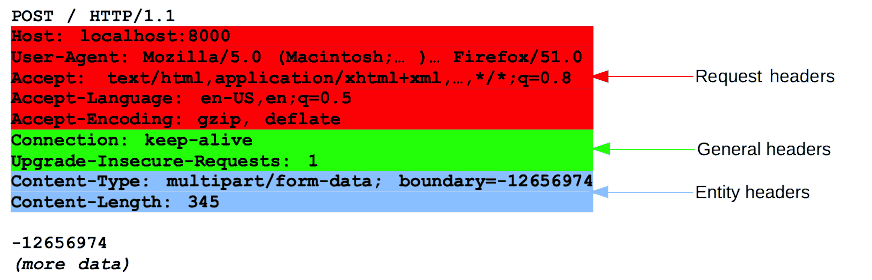
\includegraphics[width=\textwidth,keepaspectratio=true]{images/HTTP-request-headers.png}
          \caption[Các thành phần trong tiêu đề của một \acrshort{http} request]{Các thành phần trong tiêu đề của một \acrshort{http} request \protect\parencite{mdn-HTTP-message}}
          \label{fig:HTTP-request-headers}
        \end{figure}
        \begin{itemize}
            \item \textbf{Tiêu đề chung (general headers)} gồm những quy tắc/phiên bản được áp dụng lên toàn bộ request.
            \item \textbf{Tiêu đề request (request headers)} làm rõ request bằng việc đặc tả kĩ hơn về bối cảnh yêu cầu cũng như những giới hạn có điều kiện trên request đó.
            \item \textbf{Tiêu đề thực thể (entity headers)} gồm những quy tắc áp dụng lên phần nội dung (body) của request, nếu request không có nội dung thì phần tiêu đề cũng không có những tiêu đề thực thể này.
        \end{itemize}
    \item \textbf{Nội dung (body)} được phân cách với phần tiêu đề bởi một dòng trống. Phần nội dung này có thể có hoặc không, đa phần nó hiện diện trong những request có phương thức \texttt{POST} được gửi kèm theo biểu mẫu dữ liệu HTML.
\end{itemize}
\textbf{Thông báo phản hồi HTTP} (HTTP response) được máy chủ trả về  cho người dùng, là câu trả lời cho hành động đã được yêu cầu bởi người dùng thông qua \acrshort{http} request. \acrshort{http} response gồm các thành phần tương tự như HTTP request. Các dòng tiêu đề trên \acrshort{http} response cũng được phần làm 3 loại chính như Hình \ref{fig:HTTP-response-headers} sau.
\begin{figure}[H]
  \centering
    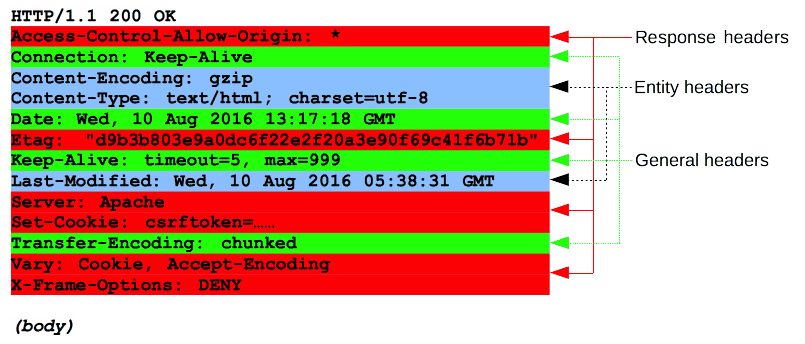
\includegraphics[width=\textwidth,keepaspectratio=true]{images/HTTP-response-headers.png}
  \caption[Các thành phần trong tiêu đề của một \acrshort{http} response]{Các thành phần trong tiêu đề của một \acrshort{http} response \protect\parencite{mdn-HTTP-message}}
  \label{fig:HTTP-response-headers}
\end{figure}

% TODO: có thế sẽ viết thêm về cả CSP và CORS?
\subsection{Chính sách cùng nguồn gốc}
Phần này trình bày khái niệm và những ngoại lệ của chính sách cùng nguồn gốc \parencite{sullivan2011web} \acrfull{sop}. Chính sách cùng nguồn gốc là một trong những khái niệm nền tảng trong lĩnh vực bảo mật trình duyệt web. Không có \acrshort{sop} thì mọi trang web trên internet đều có thể tiếp cần được thông tin bí mật của người dùng ở bất kì trang web nào khác. Việc khai thác các lỗ hổng bảo mật như \acrshort{xss}, \acrshort{sqli} (sẽ được làm rõ ở phần sau), \acrfull{xsrf},... là cách thức chủ yếu để vượt qua tính phòng thủ vốn có của \acrshort{sop}. \acrshort{sop} là một sự đồng thuận cần thiết giữa những nhà cung cấp trình duyệt web (như Microsoft, Apple, Google, Mozilla, Opera) trong việc giới hạn chức năng cũng như quyền hạn của các đoạn mã kịch bản (scripting code) trên trình duyệt của \textbf{người dùng} (client-side, phân biệt với phía máy chủ - server-side). \acrshort{sop} quy định rằng khi người dùng đang truy cập một trang web X nào đó trên trình duyệt, những đoạn mã của trang web X đó chỉ được phép đọc và ghi nội dung xuống một trang web Y khác (và ngược lại) nếu cả hai trang web X và Y có cùng nguồn gốc (origin). Hai trang web có cùng nguồn gốc ở đây có nghĩa là giống hệt nhau về ba thành phần: giao thức tầng ứng dụng của trang web (\acrshort{http}, \acrshort{https}), cổng TCP (thường là cổng 80 cho giao thức \acrshort{http} và cổng 443 cho giao thức \acrshort{https}), và tên miền của hai trang web (ví dụ \texttt{www.example.com} hay \texttt{www.google.com}).
\begin{figure}[H]
  \centering
    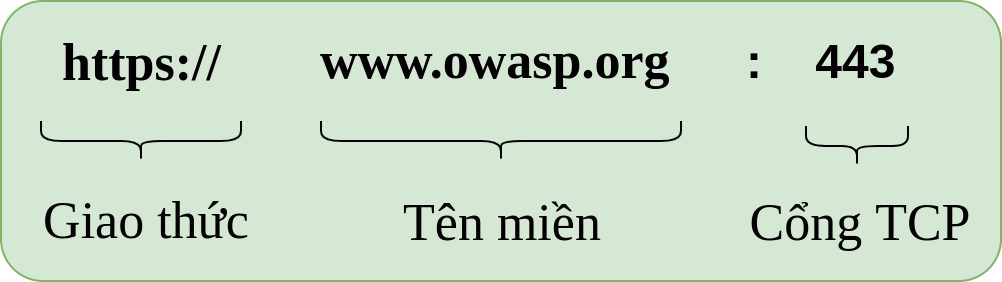
\includegraphics[width=0.6\textwidth,keepaspectratio=true]{images/origin-definition.png}
  \caption{Các thành phần của nguồn gốc (origin) của một trang web}
  \label{fig:origin-definition}
\end{figure}
Ví dụ về việc so sánh nguồn gốc giữa các trang web khác nhau được thể hiện như Bảng \ref{tab:SOP-example} sau.
\begin{table}[ht]
    \centering
    \caption{Minh họa việc so sánh nguồn gốc với trang web \texttt{https://drive.google.com/my-drive}}
    \label{tab:SOP-example}
    \begin{tabular}[t]{lcc}
        \toprule[1pt]\midrule[0.3pt]
            \textbf{Đường dẫn URL}&\textbf{Kết quả}&\textbf{Lý do}\\
        \midrule
            \texttt{https://drive.google.com/your-drive}&Cùng nguồn gốc&Chỉ khác đường dẫn\\
            \addlinespace
            \texttt{https://drive.google.com/my-drive/my-docs}&Cùng nguồn gốc&Chỉ khác đường dẫn\\
            \addlinespace
            \texttt{http://drive.google.com/my-drive}&Không cùng nguồn gốc&Khác giao thức\\
            \addlinespace
            \texttt{https://drive.google.com:444/my-drive}&Không cùng nguồn gốc&Khác cổng\\
            \addlinespace
            \texttt{https://mail.google.com/my-drive}&Không cùng nguồn gốc&Khác tên miền\\
        \midrule[0.3pt]\bottomrule[1pt]
    \end{tabular}
\end{table}
Bên cạnh việc chỉ cho phép tương tác về mặt dữ liệu với những trang web có cùng nguồn gốc thì \acrshort{sop} cũng có một số ngoại lệ, cho phép ứng dụng web vượt qua \acrshort{sop} một cách có kiểm soát. Điều này giúp ứng dụng web trở nên uyển chuyển, giàu nội dung, đa chức năng và dễ hiện thực các chức năng đó hơn. Một số thẻ \acrshort{html} ngoại lệ được vượt qua \acrshort{sop} tiêu biểu có thể kể đến.
\begin{itemize}
    \item \texttt{<script src="..."></script>}
    \item \texttt{<link rel="stylesheet" href="...">}
    \item \texttt{<img src="...">, <video>, <audio>, <object>, <applet>}
    \item \texttt{<iframe src="...">, <frame>}
\end{itemize}
Những thẻ \acrshort{html} kể trên (cùng với một số ngoại lệ đặc thù khác) được phép tải về và thực thi mã nguồn/hình ảnh/video từ địa chỉ web được đặc tả trong thuộc tính \texttt{src}, \texttt{href},... cho dù những địa chỉ web đó có thể không có cùng nguồn gốc với trang web nguồn.
